\documentclass{beamer}
\usepackage{pgfpages}
\usepackage{amsmath}
\usepackage{tikz}
\usetikzlibrary{shapes.geometric}
\usetikzlibrary{positioning}
\usepackage{graphicx}
\usepackage{bbding}
\defbeamertemplate{itemize item}{raisedsquare}{\rule[0.5ex]{0.6ex}{0.6ex}}
\defbeamertemplate{itemize item}{boldarrow}{\ArrowBoldRightShort}
%\pgfpagesuselayout{4 on 1}[a4paper,border shrink=5mm,landscape]

% \usetheme{Warsaw}
% \usecolortheme{crane}
\useinnertheme{rectangles}
\useoutertheme{tree}
\usefonttheme{serif}


\tikzset{darkstyle/.style={circle,draw,fill=gray!40}}

\begin{document}
    
    \begin{frame}{Fibonacci heap: Extract Min}
        \begin{tikzpicture}[
    rd1/.style={circle, draw=black!60, fill=red!50, very thick, minimum size=4mm},
    rd2/.style={circle, draw=black!60, fill=blue!50, very thick, minimum size=4mm},
    rd3/.style={circle, draw=black!60, fill=black!50, very thick, minimum size=4mm}
    ]
            \node[rd1] (n3) {3};
            \node[rd2] (n17) [left = of n3] {17};
            \node[rd2] (n23) [left = of n17] {23};
            \node[rd2] (n24) [left = of n23] {24};
            \node[rd2] (n7) [left = of n24] {7};
            
            \node[rd2] (n46) at [below = of n24] {46};
            
            
            \node[rd2] (n30) [below = of n7] {30};
            %node[rd3] (n26) [below of n24] {26};
            
            \draw[dotted, -] (n3.west) -- (n17.east);
            \draw[dotted, -] (n17.west) -- (n23.east);
            \draw[dotted, -] (n23.west) -- (n24.east);
            \draw[dotted, -] (n24.west) -- (n7.east);
            
            \draw[-] (n7.south) -- (n30.north);
            \draw[-] (n24.south) -- (n46.north);
                
            \end{tikzpicture}
    \end{frame}

    \begin{frame}{Fibonacci: text and image}
        \begin{columns}
            \begin{column}{0.5\textwidth}
            \begin{itemize}
                    \item[\dot]Extract/delete min \pause
                    \begin{itemize}
                        \item Delete min and add its children into the root list
                        \item Consolidate trees so that no two roots have same degree
                    \end{itemize}
                \end{itemize}

            \end{column}
            \begin{column}{0.5\textwidth}  %%<--- here
                \begin{center}
                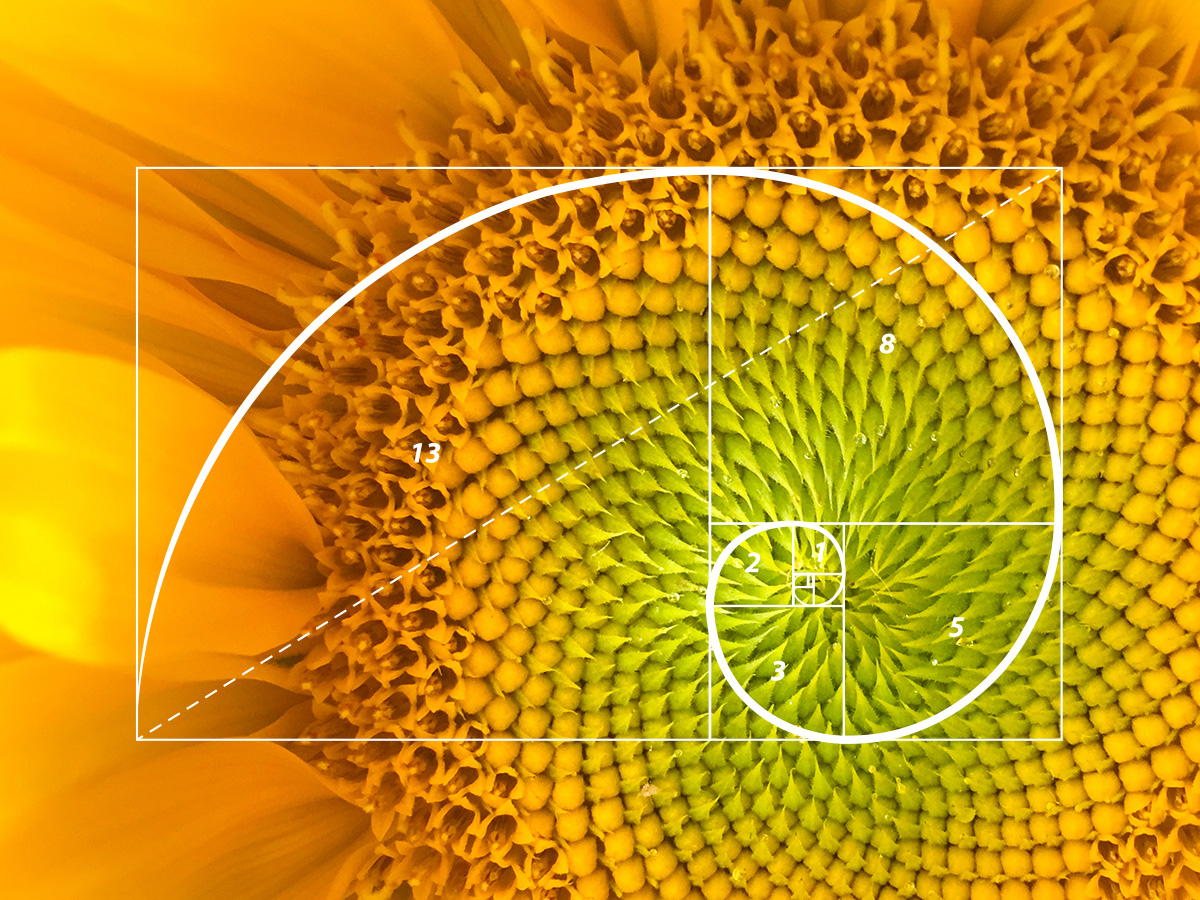
\includegraphics[width=0.9\textwidth]{the-golden-ratio-teaser.jpg}
                \end{center}
            \end{column}
        \end{columns}
    \end{frame}

\end{document}
